\chapter{Marktumgebung}

\section{Kundenseitige Entwicklungen}

Da die Preise für die europäischen Emissionszertifikate (EU-ETS) in naher Zukunft voraussichtlich steigen werden und positive Nettoemissionen letztendlich ganz verboten werden, werden die Kunden einen höheren Gewinn aus einer Investition erzielen, die ihr Nettoemissionsprofil reduziert.
Ab Februar 2024 werden die Emissionszertifikate pro Tonne CO2 mit 68 € bewertet (siehe Abbildung unten).
Ab Februar 2024 wird der Preis der Emissionszertifikate pro Tonne CO2 auf 68 € festgesetzt.
Dieser Preis unterliegt der Marktdynamik und regulatorischen Änderungen.
Der Trend deutet auf einen stetigen Anstieg der Kosten für Emissionszertifikate hin, der durch eine strengere Klimapolitik und eine sinkende Obergrenze für die Gesamtemissionen bedingt ist.
Dieser Aufwärtstrend dürfte sich fortsetzen und spiegelt das Engagement der EU zur Erreichung ihrer Klimaziele wider.

\begin{figure}[h]
    \centering
    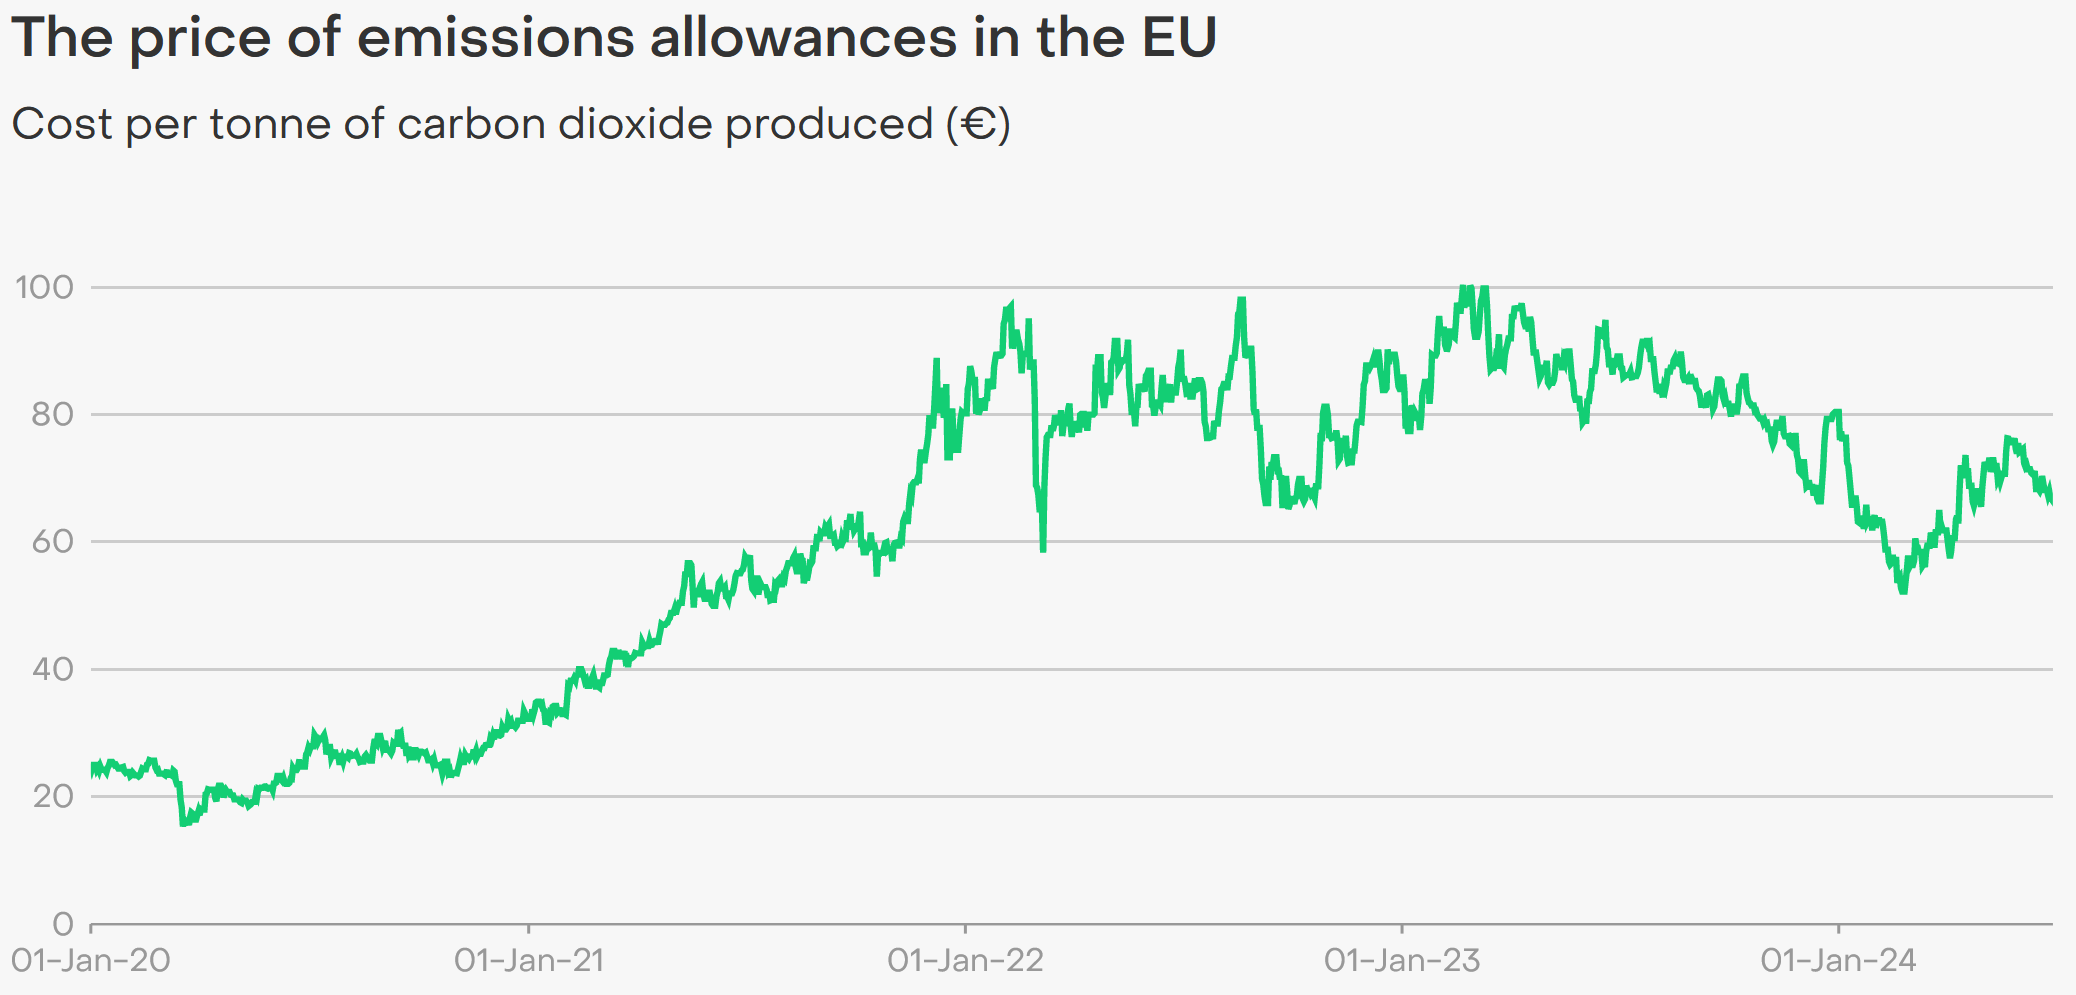
\includegraphics[width=.9\textwidth]{Carbon Price Tracker_Ember.png}
    \label{fig:carbon price tracker}
    \caption[Entwicklung der CO2-Bepreisung in der EU]{Entwicklung der CO2-Bepreisung in der EU von 2020 bis heute.}
\end{figure}

Das regulatorische Umfeld wird immer strenger, und es wird erwartet, dass Nettoemissionen in naher Zukunft gänzlich verboten werden.
Dieser regulatorische Druck zwingt die Unternehmen dazu, nach innovativen Lösungen zu suchen, um ihren Kohlenstoff-Fußabdruck zu verringern.
In Anbetracht der steigenden Kosten für Emissionszertifikate und der sich verschärfenden rechtlichen Rahmenbedingungen können die Kunden erhebliche finanzielle Vorteile aus Investitionen in Technologien ziehen, die ihr Nettoemissionsprofil reduzieren.
Durch den Einsatz von ALGAALGAs fortschrittlichen Systemen zur Kohlenstoffabscheidung und -nutzung können Kunden:

\begin{enumerate}
    \item Reduzieren Sie die Emissionskosten: Senkung ihrer Ausgaben für Emissionszertifikate durch Verringerung ihrer Netto-Kohlendioxidemissionen.
    \item Verbesserung der Rentabilität: Verbessern Sie ihr Endergebnis, indem Sie die finanziellen Auswirkungen der steigenden Preise für Emissionszertifikate abmildern.
    \item Einhaltung von Vorschriften: Sicherstellung der Einhaltung aktueller und zukünftiger gesetzlicher Vorschriften, Vermeidung von Strafen und Verbesserung des Rufs des Unternehmens.
    \item Nachhaltige Praktiken: Demonstration des Engagements für Nachhaltigkeit, was den Markenwert steigern und umweltbewusste Kunden und Investoren anziehen kann.
\end{enumerate}

Die steigenden Kosten für Emissionszertifikate und das drohende Verbot positiver Netto-Emissionen bieten ALGAALGA eine große Marktchance.
Unternehmen aus verschiedenen Sektoren, darunter die verarbeitende Industrie, der Energiesektor und die Landwirtschaft, suchen aktiv nach kostengünstigen und effizienten Lösungen, um ihren Kohlenstoff-Fußabdruck zu verwalten.
ALGAALGAs modulare Mikroalgen-Bioreaktoren bieten eine skalierbare und vielseitige Lösung, die diesen Anforderungen gerecht wird.
Durch die Positionierung als führendes Unternehmen im Bereich der Kohlenstoffabscheidung und -verwertung ist ALGAALGA gut positioniert, um von der wachsenden Nachfrage nach nachhaltigen und konformen Lösungen zur Emissionsreduzierung zu profitieren.
Unsere Technologie erfüllt nicht nur die unmittelbaren Bedürfnisse unserer Kunden, sondern bietet auch langfristige Vorteile, indem sie zu einer nachhaltigen und kohlenstoffneutralen Zukunft beiträgt.

\begin{figure}[h]
    \centering
    \includesvg[width=.9\textwidth]{biofuel_prod}
    \label{fig:biofuel production}
    \caption[Entwicklung des Produktionsvolumens von Biotreibstoff]{Entwicklung des Produktionsvolumens von Biotreibstoff.}
\end{figure}